\section{Derivation of a MOSFET Small Signal Model}
\begin{frame}{Derivation: Notational Conventions}
    \begin{itemize}
        \item DC quantities are labeled with UPPERCASE variables and UPPERCASE subindices: 
        $V_{\mathrm{GS}}$
        \item Pure AC quantities are labeled with lowercase variables and lowercase subindices: 
        $v_{\mathrm{gs}}$
        \item Superpositions of both quantities are labeled with lowercase variables and 
        UPPERCASE subindices: $v_{\mathrm{GS}}=V_{\mathrm{GS}}+v_{\mathrm{gs}}$

        \begin{figure}
            \centering
            \includegraphics{../plots/notational_convention.pdf}
            \caption{Notational conventions for DC and AC quantities.}
            \label{fig:signal_convention}
        \end{figure}
    \end{itemize}
\end{frame}

\begin{frame}{Derivation: MOSFET Current-Voltage Characteristics}
    \vspace{0.5cm}
    \begin{figure}
        \centering
        \includegraphics{../plots/cv_characteristics.pdf}
        \caption{MOSFET current-voltage characteristics.}
        \label{fig:mosfet_characteristics}
    \end{figure}
    \begin{itemize}
        \item Require saturation-region operation: $V_{\mathrm{DS}}\gg V_{\mathrm{GS}}-V_{\mathrm{t}}$
        \item In this regime, the following current-voltage characteristics are valid:
            \begin{itemize}
                \item $i_{\mathrm{drain}}=\frac{1}{2}k_{\mathrm{n}}(v_{\mathrm{gate}}-V_{\mathrm{t}})^{2}$
                \item $i_{\mathrm{gate}}=0$
            \end{itemize}
    \end{itemize}
\end{frame}

\begin{frame}{Derivation: Signal Current in Drain Terminal}
    \begin{itemize}
        \item Apply a signal $v_{\mathrm{GS}}=V_{\mathrm{GS}}+v_{\mathrm{gs}}$ to the gate terminal.
        \item This results in the following drain current:
    \end{itemize}
    \begin{block}{}
        \setlength{\abovedisplayskip}{0pt}
        \setlength{\belowdisplayskip}{0pt}
        \begin{align*}
            i_{\mathrm{D}}&=\frac{1}{2}k_{\mathrm{n}}(V_{\mathrm{GS}}+v_{\mathrm{gs}}
            -V_{\mathrm{t}})^{2} \\
            &=\underbrace{ \frac{1}{2}k_{\mathrm{n}}(V_{\mathrm{GS}}-V_{\mathrm{t}})^{2} }_{ =I_{\mathrm{D}}}+
            k_{\mathrm{n}}(V_{\mathrm{GS}}-V_{\mathrm{t}})v_{\mathrm{gs}}
            +\frac{1}{2}k_{\mathrm{n}}v_{\mathrm{gs}}^{2}
        \end{align*}
    \end{block}
    \begin{itemize}
        \item The third term is negligible for sufficiently small $v_{\mathrm{gs}}$, i.e. 
        $v_{\mathrm{gs}}\ll 2(V_{\mathrm{GS}}-V_{\mathrm{t}})$.

    \end{itemize}
\end{frame}

\begin{frame}{Derivation: Signal Current in Drain Terminal}
    \begin{block}{}
        \begin{itemize}
            \item Neglecting the third term under the specified condition results in the following 
            expression for the drain current $i_{\mathrm{D}}$:
        \end{itemize}
        \begin{align*}
                i_{\mathrm{D}}&=I_{\mathrm{D}}+i_{\mathrm{d}} \\
                I_{\mathrm{D}}&=\frac{1}{2}k_{\mathrm{n}}(V_{\mathrm{GS}}-V_{\mathrm{t}})^{2} \\
                i_{\mathrm{d}}&=k_{\mathrm{n}}(V_{\mathrm{GS}}-V_{\mathrm{t}})v_{\mathrm{gs}}
        \end{align*}
    \end{block}

    \begin{itemize}
        \item the parameter, that related $i_{\mathrm{d}}$ and $v_{\mathrm{gs}}$ is called the 
        transconductance $g_{\mathrm{m}}=k_{\mathrm{n}}(V_{\mathrm{GS}}-V_{\mathrm{t}})$ 
    \end{itemize} 
\end{frame}

\begin{frame}{Derivation: Linear Circuit}
    \begin{itemize}
        \item A linear circuit is a circuit that obeys the superposition principle:
        \begin{itemize}
            \item Let the output of the circuit be $F(x)$.
            \item Let the input signal be a linear combination $a x_{1}(t)+b x_{2}(t)$.
            \item The circuit satisfies $F(a x_{1}(t) + b x_{2}(t)) = a F(x_{1}(t)) + b F(x_{2}(t))$.
        \end{itemize}
        \item Circuits made of ideal resistors, capacitors, inductors, voltage- and current sources are linear circuits.
        \item Circuits are nonlinear if they have nonlinear components (e.g., diodes, transistors).
        \item When small signals are applied, transistors tend to behave approximately linearly:
        \begin{itemize}
            \item They can be replaced with a small signal model.
            \item This allows the use of linear analysis techniques.
        \end{itemize}
    \end{itemize}
    \note[item]{Other components, whole digital logic circuits}
\end{frame}

\begin{frame}{Deviation: Small-Signal Equivalent Circuit}
    \begin{itemize}
        \item Signal analysis can be simplified by separating DC calculation from small-signal calculation.
        \item Only care about the signal components and assume one steady bias point.
        \item From the preceding analysis, we get the following equations.
        \begin{itemize}
            \item $i_{\mathrm{g}}(v_{\mathrm{gs}}, v_{\mathrm{ds}})=0$ \\
            \item $i_{\mathrm{d}}(v_{\mathrm{gs}}, v_{\mathrm{ds}})=g_{\mathrm{m}}v_{\mathrm{gs}}$
        \end{itemize}
        \item A circuit that satisfies these equations is called a small-signal equivalent circuit.
    \end{itemize}
\end{frame}

\begin{frame}{Deviation: Small-Signal Equivalent Circuit}
    \begin{figure}
        \centering
        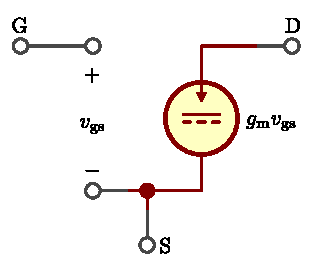
\includegraphics{../assets/small_signal.pdf}
        \caption{Small-signal equivalent circuit of a MOSFET.}
        \label{fig:mosfet_small_signal_model}
    \end{figure}
\end{frame}